\chapter{Développement Android}

\section{La capture de points sous Android}
\label{capture de points}
Sous Android, la localisation d'un appareil utilisant une puce GPS est rendue possible. Bien évidemment, plus la puce est performante, plus la localisation de l’appareil sera rapide. La capture de points se fait grâce à trois fournisseurs (\textit{providers}) différents.

\subsection{Les \textit{providers}}
Nous parlerons ici uniquement des providers nécessaire au fonctionnement de notre application à savoir le \textit{NETWORK\_PROVIDER} et \textit{GPS\_PROVIDER} cependant un récapitulatif des providers est disponible à l'Annexe \ref{Annexe2}.

\subsubsection{Le \textit{NETWORK\_PROVIDER}}
Ce fournisseur détermine la position de l'appareil en fonction des antennes téléphoniques et des points d'accès au Wi-fi. Il a une précision d'environ 60 mètres mais fournit des points beaucoup plus rapidement que le GPS. Nous l'utilisons dans notre application le temps que la puce se synchronise avec le GPS.

\subsubsection{Le \textit{GPS\_PROVIDER}}
De tous les fournisseurs, celui-ci est de loin de plus précis puisqu'il permet de localiser un appareil avec une précision de 6 mètres. Malheureusement, pour se faire, la puce de l'appareil doit se connectée à un GPS est cela peut prendre beaucoup de temps. De plus, tant que l'acquisition n'a pas été établie, aucun point ne sera fourni.

\begin{note}
L'utilisation du service de localisation sous Android nécessite des permissions que l'on doit ajouter au \textit{manifest} (Partie \ref{manifest}).
\end{note}

\subsection{Le LocationManager}
\label{locationManager}
Le \verb!LocationManager! représente le service de gestion de capture de points. C'est grâce à cette classe que l'acquisition de points peut se faire. Son fonctionnement est brièvement représenté par le diagramme \ref{Diagramme Location Manager}. Son instanciation se fait grâce aux services Android. Une fois l'instance obtenue, l'appel à la méthode \verb!requestLocationUpdates! doit être fait en précisant le \textit{provider} utilisé ainsi que deux variables et un \verb!LocationListener!. Les deux variables correspondent au minimum de temps et de distance nécessaire avant la capture d'un nouveau point. La valeur de ces variables est inversement proportionnelle à la consommation de la batterie. À chaque fois qu'un nouveau point est trouvé, le \verb!LocationListener!, qui écoute l'arrivée d'une nouvelle \verb!Location!, va pouvoir l'ajouter  à la liste des points du trajet. C'est également le \verb!LocationListener! qui va vérifier la bonne continuité du signal. En cas de modification, de perte ou de récupération du signal, un appel est effectué via les méthodes correspondantes.

\begin{img}  
	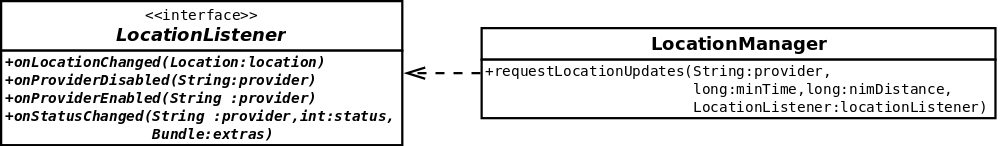
\includegraphics[scale=0.65]{img/LocationManager.png}
	\caption{Fonctionnement du Location Manager}
	\label{Diagramme Location Manager}
\end{img}

\section{Les différents composants d'Android}
Google met à disposition des développeurs un kit de développement (SDK) complet et une API (interface de développement) très bien documentée pour développer des applications Android. Nous allons voir dans cette partie les bases du développement sous Android et ses différents composants.
\subsection{Les activités}
Les applications Android fonctionnent avec ce que l'on appelle des activités (classe \verb!Activity!) et des fragments (\verb!Fragment!).
Une activité représente la totalité du contenu affiché à l'écran. Pour créer une nouvelle activité on implémente  une classe Java qui va étendre la classe \verb!Activity!. Les activités ne peuvent échanger entre elles que des paramètres de types primitifs (booléens, caractères, entiers...) et des chaînes de caractères. Pour pouvoir afficher le contenu souhaité dans une nouvelle activité nous devons donc lui passer les identifiants des objets à traiter sous forme d'entier (par exemple l'identifiant du trajet à afficher).\bigskip

La Figure \ref{cycle de vie} explique le cycle de vie d'une activité avec les différentes méthodes appelées à chaque événement. Ce diagramme nous a été très utile pour comprendre la mécanique de transition entre les activités. En effet, lorsqu'une nouvelle activité est instanciée, la précédente se met dans une pile d'activités et continue à consommer les ressources du système. Il est donc plus que nécessaire de connaître le traitement à effectuer en fonction de chaque cas.

\begin{img}
  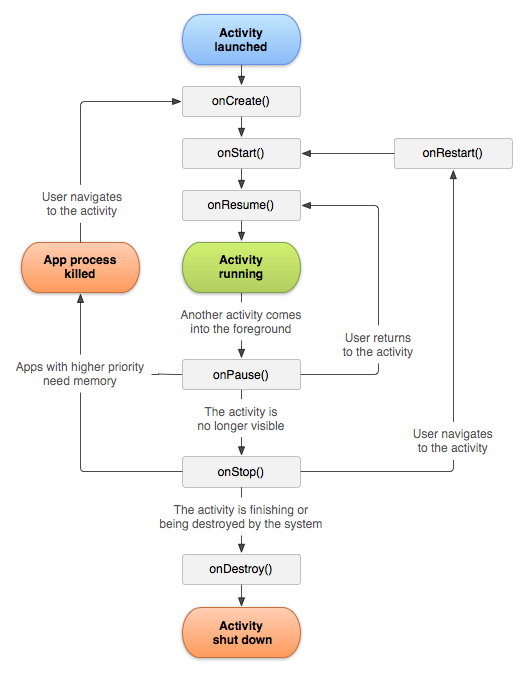
\includegraphics[scale=0.5]{img/cycle.png}
  \caption{Cycle de vie d'une Activity}
  \label{cycle de vie}
\end{img}

Les méthodes les plus importantes dans notre développement sont:\bigskip
 \begin{itemize}
 	\item \verb!onCreate()! lancé au démarrage de l'activité. C'est ici que l'on peux récupérer les valeurs passées en paramètre à l'activité et ainsi instancier les objets nécessaires.
 	\item \verb!onRestart()! lancé lorsque l'utilisateur utilise la touche précédent de son smartphone. L'activité dans la pile d'activités, déjà instanciée une première fois, doit alors vérifier les données à mettre à jour pour actualiser l'affichage.
 \end{itemize}

\subsection{Les fragments}
Les fragments (classe \verb!Fragment!) sont des sous-activités qui peuvent être intégrés dans une activité (par exemple une liste ou une boite de dialogue). Ils possèdent le même cycle de vie que les activités à l'exception de deux méthodes supplémentaires:\bigskip
 
\begin{itemize}
 	\item \verb!onAttach()! appelée lorsque le fragment est attaché à une activité, juste avant la méthode \verb!onCreate()! ce qui lui permet en général de vérifier que l'activité est compatible et implémente bien les bonnes interfaces.
 	\item \verb!onDetach()! appelée après la méthode \verb!onDestroy()!.
\end{itemize}\bigskip

Plusieurs fragments peuvent être attachés à une activité. Pour communiquer entre eux ils doivent impérativement passer par l'activité qui les contient à travers des méthodes de callback. Il est donc conseiller de définir des interfaces internes aux fragments que les activités qui sont amenées à les contenir doivent implémenter. 

\subsection{Les ressources}
Les ressources représentent toutes les données statiques que l'application va contenir. Elles sont accessibles à partir de n'importe quelle activité à l'aide d'une classe nommée \verb!R!. Cette classe est très spéciale. En effet, c'est à la compilation du projet que cette classe est créée. Le système parcours alors toutes les ressources et insère une référence statique dans cette classe pour chacune d'entre elles.\bigskip
Il existe plusieurs types de ressources :\bigskip

\begin{itemize}
 	\item les \verb!layouts!
 	\item les \verb!values!: des fichiers XML qui stockent les chaines de caractères
 	\item les \verb!drawable!: toutes les images
\end{itemize}\bigskip

\subsubsection{Les layouts}
Chaque activité (et fragment) peut être associée à un layout pour afficher des éléments graphiques à l'écran. Un layout est une ressources sous forme de fichier XML dans lequel on déclare les composants graphiques (objets \verb!View()!) à afficher. Pour insérer une donnée dans ce layout il faut, à partir de l'activité ou du fragment, récupérer l'objet \verb!View! adéquat et lui assigner la donnée qu'il doit contenir. \bigskip

Les principaux composants que l'on a utilisé dans nos layouts sont:\bigskip

\begin{itemize}
 	\item \verb!TextView! qui permet d'afficher un texte.
 	\item \verb!Button! qui affiche un bouton cliquable.
 	\item \verb!ListView! qui permet de créer une liste d'objets cliquables.
\end{itemize}\bigskip
 
Le code \ref{le layout} donne un aperçu d'un fichier layout contenant un texte avec un fragment de type \verb!GoogleMap! ordonnés verticalement dans l'écran.
\begin{xml}[Exemple d'un layout]
<?xml version="1.0" encoding="utf-8"?>
<LinearLayout xmlns:android="http://schemas.android.com/apk/res/android"
    android:orientation="vertical" android:layout_width="match_parent"
    android:layout_height="match_parent">	
	<TextView
		android:id="@+id/textView"
    	android:layout_width="match_parent"
        android:layout_height="match_parent"        
        android:layout_weight="0.5"
        android:text="@string/temps" />
    <fragment
        android:id="@+id/map_container"
        android:layout_width="fill_parent"
        android:layout_height="fill_parent"
        android:layout_weight="0.5"
        class="com.google.android.gms.maps.SupportMapFragment" />
</LinearLayout>
\end{xml}
\label{le layout}

\subsection{L'Android manifest}
\label{manifest}

L'android \verb!manifest! est le fichier de configuration globale. Ce fichier XML déclare toutes les activités, la version minimale d'Android compatible avec l'application et surtout les permissions nécessaires au bon fonctionnement de l'application. Les permissions dont notre application a besoin sont les suivantes:\bigskip

\begin{itemize}
 	\item \verb!ACCESS_FINE_LOCATION! permet d'accéder à la localisation précise du smartphone.
 	\item \verb!WRITE_EXTERNAL_STORAGE! permet de créer des fichiers, en l'occurrence des fichiers GPX.
 	\item \verb!READ_EXTERNAL_STORAGE! permet de lire les fichiers externes.
 	\item \verb!INTERNET! accès à Internet pour l'affichage de la carte.
\end{itemize}\bigskip

\section{Structure du projet}

Tout au long de notre développement, nous avons essayé de séparer au maximum les différents composants de l'application pour obtenir un code propre et surtout réutilisable. On peut voir dans l'architecture ci-dessous comment sont organisés les fichiers. On a une partie Java qui va contenir les différentes classes et une autre qui va contenir toutes les ressources.\bigskip

\begin{img}
  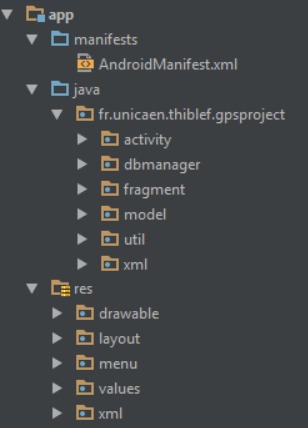
\includegraphics[scale=0.45]{img/archi.png}
  \caption{Architecture de l'application}
\end{img}

Notre application suit le patron de conception MVC (Modèle, Vue, Contrôleur). Les ressources représentent la vue, les activités et fragments représentent les contrôleurs et les packages restants représentent le modèle de l'application.\bigskip

Décrivons rapidement les différents paquetages:\bigskip

\begin{itemize}
 	\item \verb!activity! contient toutes les activités de l'application.
 	\item \verb!dbmanager! contient les classes de création et d'accès à la base de données.
 	\item \verb!fragment! contient tous les fragments.
 	\item \verb!model! contient les classes modèles (\verb!Parcours!, \verb!Trajet!).
 	\item \verb!util! contient des classes utilitaires permettant notamment de convertir les différentes données (par exemple de convertir des mètres par seconde en kilomètres par heure).
 	\item \verb!xml! contient toutes les classes nécessaires au stockage et à la lecture des données GPS dans les fichiers GPX.
\end{itemize}\bigskip
 



